\chapter{Memory Management Concepts}
\label{chapter:memmgmt}

Throughout the lifetime of a process its memory requirements change. Whether the process has to create more objects or allocate arrays or even temporary variables, it has to have a way of requesting more memory and a way to release that memory when it is no longer needed. Since our purpose is to actively monitor the exact memory consumption of a process\footnote{For simplicity, let us assume that the piece of software we are interested in monitoring runs only in one process.}, the underlying mechanisms of memory allocation and deallocation are of direct interest.  This chapter explains these mechanisms and explains how each of them are relevant to our original goals of finding out how much memory a process consumes and how different parts of that process interact with each other to reach that specific memory consumption state. The terms described in this chapter will be used throughout the rest of the thesis and they constitute the framework of our problem.

\newpage

\section{Virtual Memory}
\label{section:virtmem}

Virtual memory is a mechanism used by modern operating systems in order to give processes the illusion that there exists only one type of memory in the system which exhibits the behaviour of a directly addressable read/write memory. In addition, most operating systems run processes in separate address spaces providing the impression that processes have exclusive access to the virtual memory\footnote{There exist operating systems which use a single global address space, such as OS/VS1 and IBM i, but they still include mechanisms by which processes are stopped from accessing each other's addresses}. This is accomplished by the operating system by avoiding the direct use of physical addresses and instead making processes use logical addresses which then get translated by the operating system and the memory management unit into physical addresses. Figure \ref{fig:virtmem} shows a 32-bit system with two processes and their address spaces and the way they are mapped to physical memory and other devices.

\begin{figure}[htb]
\centering
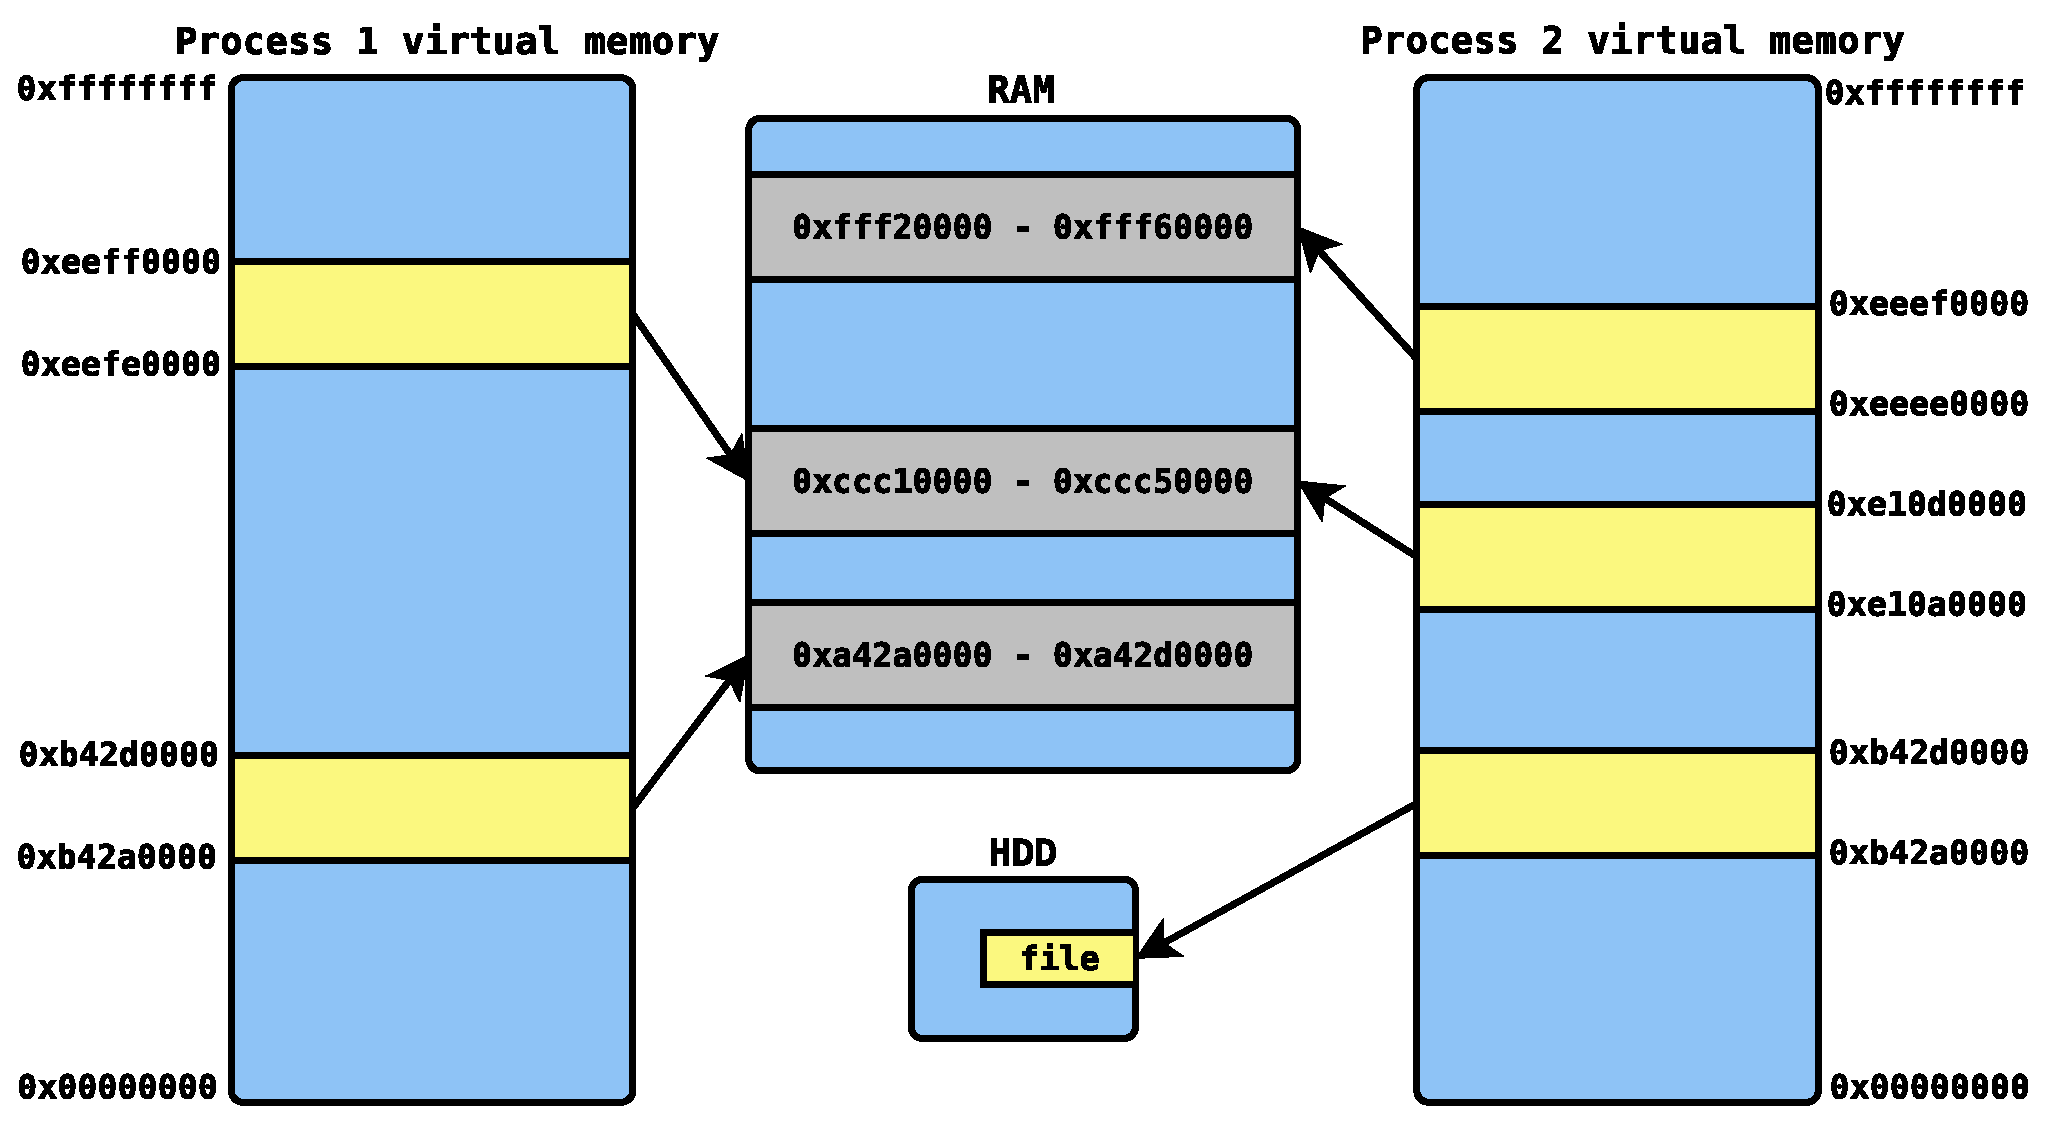
\includegraphics[width=0.8\textwidth]{src/img/virtmem}
\caption{Two processes mapping memory in diverse ways}
\label{fig:virtmem}
\end{figure}

Note that the virtual memory mechanism allows different process to share memory between each other by mapping the exact area of physical memory into possibly different areas of virtual memory and also map other devices into their address space, including files from the disk. The same virtual address in different processes can be mapped to different places, enforcing the idea of address space separation.

Monitoring a process's memory thus becomes a problem of monitoring the way its virtual memory is mapped. This leads to the question of determining which area of a process's virtual memory we are interested in monitoring. Do we monitor all of it or just specific parts? In order to answer that question we first have to understand exactly how a process's virtual memory is organized.

\section{Memory Layout}
\label{section:memlayout}

In order for a program to become a process it has to be loaded into memory\footnote{In systems with virtual memory no bytes of the program are actually copied into main memory but rather a part of the newly created process's address space is marked as containing the code. Only when the code will be executed will it be brought into main memory.} by a part of the operating system called the loader. The question is then how is the process's virtual address space organised? Several formats have existed over the years, such as Unix's a.out, MS-DOS's COM and the more recent ELF format. While these might differ drastically in terms of the object code representation, ultimately their goal is to produce a memory layout similar to Figure \ref{fig:virtmemlayout}.

\begin{figure}[htb]
\centering
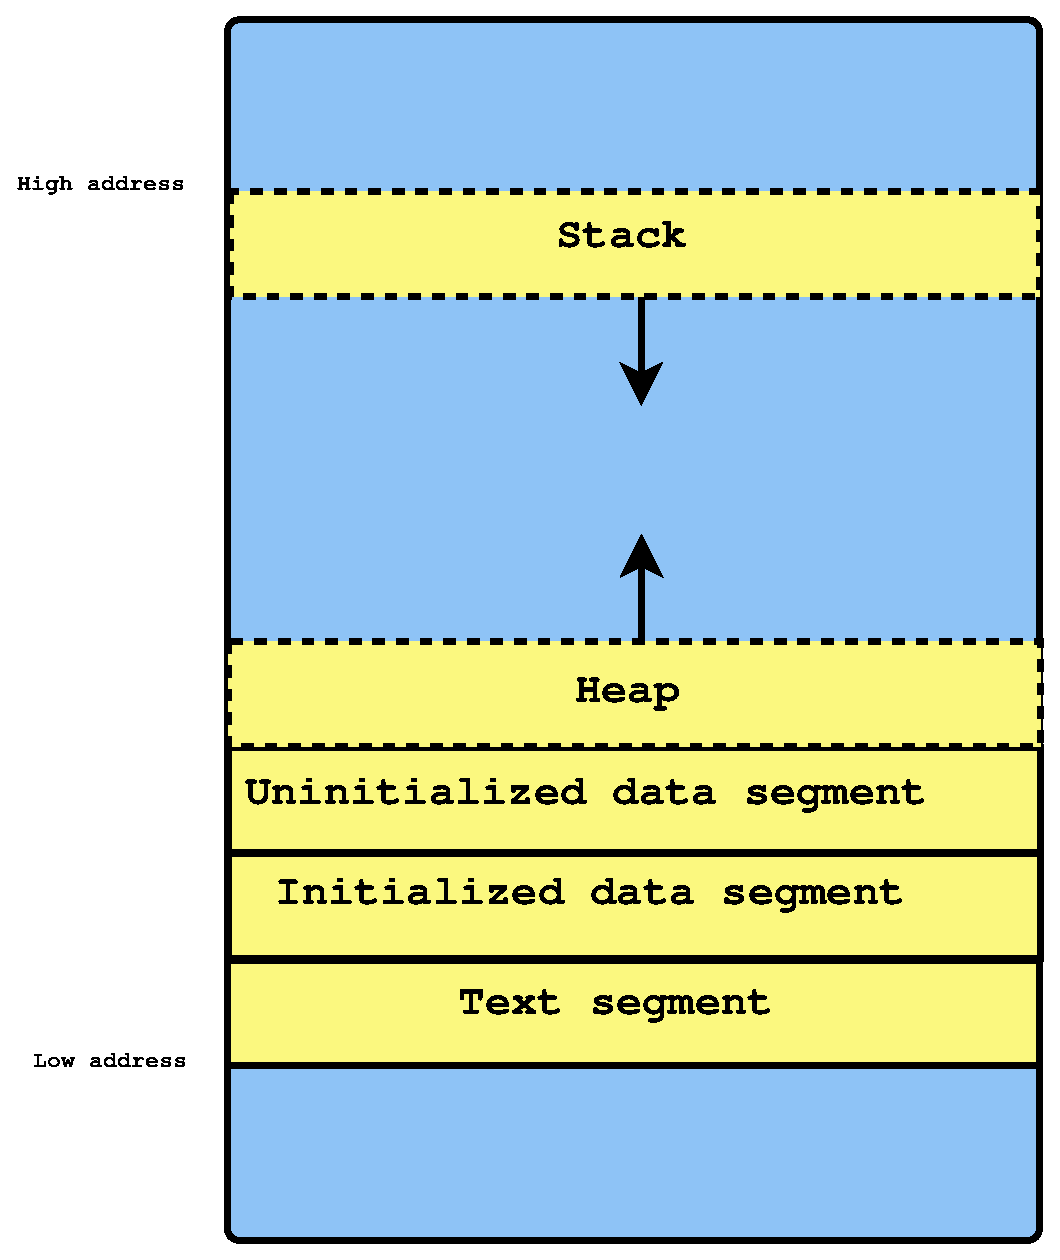
\includegraphics[width=0.4\textwidth]{src/img/virtmemlayout}
\caption{Typical virtual memory layout}
\label{fig:virtmemlayout}
\end{figure}

The segments represented are:
\begin{itemize}
\item text segment - which contains the actual code
\item initialized data segment - global variables which are initialized by the programmer
\item uninitialized data segment - variables in this segment are initialized to 0 or NULL before the program begins to execute
\item the heap - used for allocating more memory during runtime, described in section Y
\item the stack - used for function calls, as described in section X
\end{itemize}

The text segment and static data segments (initialized and uninitialized) usually do not change in size during the lifetime of a process so they are of little interestr; their size can be determined from compile time and can be reported easily. The stack and the heap, however, are constantly changing but their purpose is different. They will both help us in reaching our goal and as it will be seen in the next subchapters, ultimately we will be interested in monitoring the heap.

\section{The heap}
\label{section:heap}

The heap is where all dynamic allocations\footnote{Note that there exist system calls such as \textit{alloca} which allow dynamic allocation of space on the stack. These are rarely used and as such they won't be taken into consideration} done during the liftime of a process are stored. Operating systems offer system calls which expand the heap, thus providing access to more memory. For example, Linux offers the \textit{brk} and \textit{sbrk} system calls which change the location of the end of the process's data segment, while Windows has the \textit{*Alloc} system calls. It is however rare for high level applications to call these routines directly; instead, they use external libraries or libraries provided by the language they are written in. For example, the classical ways of allocating memory in UNIX systems makes use of the following standard C library calls:

\begin{itemize}
\item \textit{malloc/calloc} - allocates a number of bytes from the heap and return a pointer to the beginning of the block; calloc initializes this region to zero
\item \textit{realloc} - given a pointer to a previously allocated block, expand that block by a given size; it is not guaranteed that the resulting block lies in the exact place on the heap since there might not be enough contiguous space after the block
\item \textit{free} - given a pointer to a previously allocated block, release that block and mark the memory as free
\end{itemize}

Programs written in C++, even though able to call the above routines, make use of the \textit{new} and \textit{delete} operators. These operators however, in the standard C++ library, ultimately translate into calls to the above.

An additional system call available in Linux for mapping memory is \textit{mmap} which is more flexible than \textit{brk}. It allows mapping of any region of the virtual memory not only to RAM, but to files too. Given how everything in Linux is modeled as a file, including devices, mmap can basically map virtual memory to any device's internal memory as long as the latter allows it. The \textit{munmap} system call does the reverse process of unmapping virtual memory.

It is clear now that in order to monitor a process's memory consumption we have to either hook the above calls or provide wrappers around them. By doing either of these we can answer our original question of how much memory an allocation site is requesting. By allocation site we refer to a point in a program where one of the above routines/operators is invoked.

Another interesting point worth mentioning is the problem of which area of virtual memory will be selected for mapping when one of the above routines is called. It is the job of the memory allocator to selected the locations in such a way as to minimize fragmentation, maximize cache locality and provide fast allocation and deallocation speed at the same time. These goals sometimes clash and trade-offs have to be made. Techniques such as reference counting, pooling and garbage collection are sometimes used in conjunction with allocators in order to lessen the burden of memory management from the programmer. All of these have to
be taken into consideration in order to do correct memory profiling. Communication with the garbage collector, for example, might be the only way to detect when memory gets deallocated since memory is no longer explicitly released. Another example could be allocators which preallocate memory in advance so that subsequent memory allocation requests are faster. In this case we have to ask ourselves if we are interested in every mapped byte from virtual memory or just those bytes which can be potentially accessed?

\section{The stack}
\label{section:stack}

The stack is used by processes to keep track of the call chain. Each time a function is called a new stack frame is created and pushed on the stack. Upon return from that function, the stack frame is popped. A stack frame's exact structure is dependant on the platform on which the code is running, but in all cases they at least contain the following:

\begin{itemize}
\item the arguments passed to the function
\item the return address back to the caller's code
\item space for the function's local variables
\item space for the function's temporary variables in case they can not be stored in registers
\end{itemize}

\begin{figure}[htb]
\centering
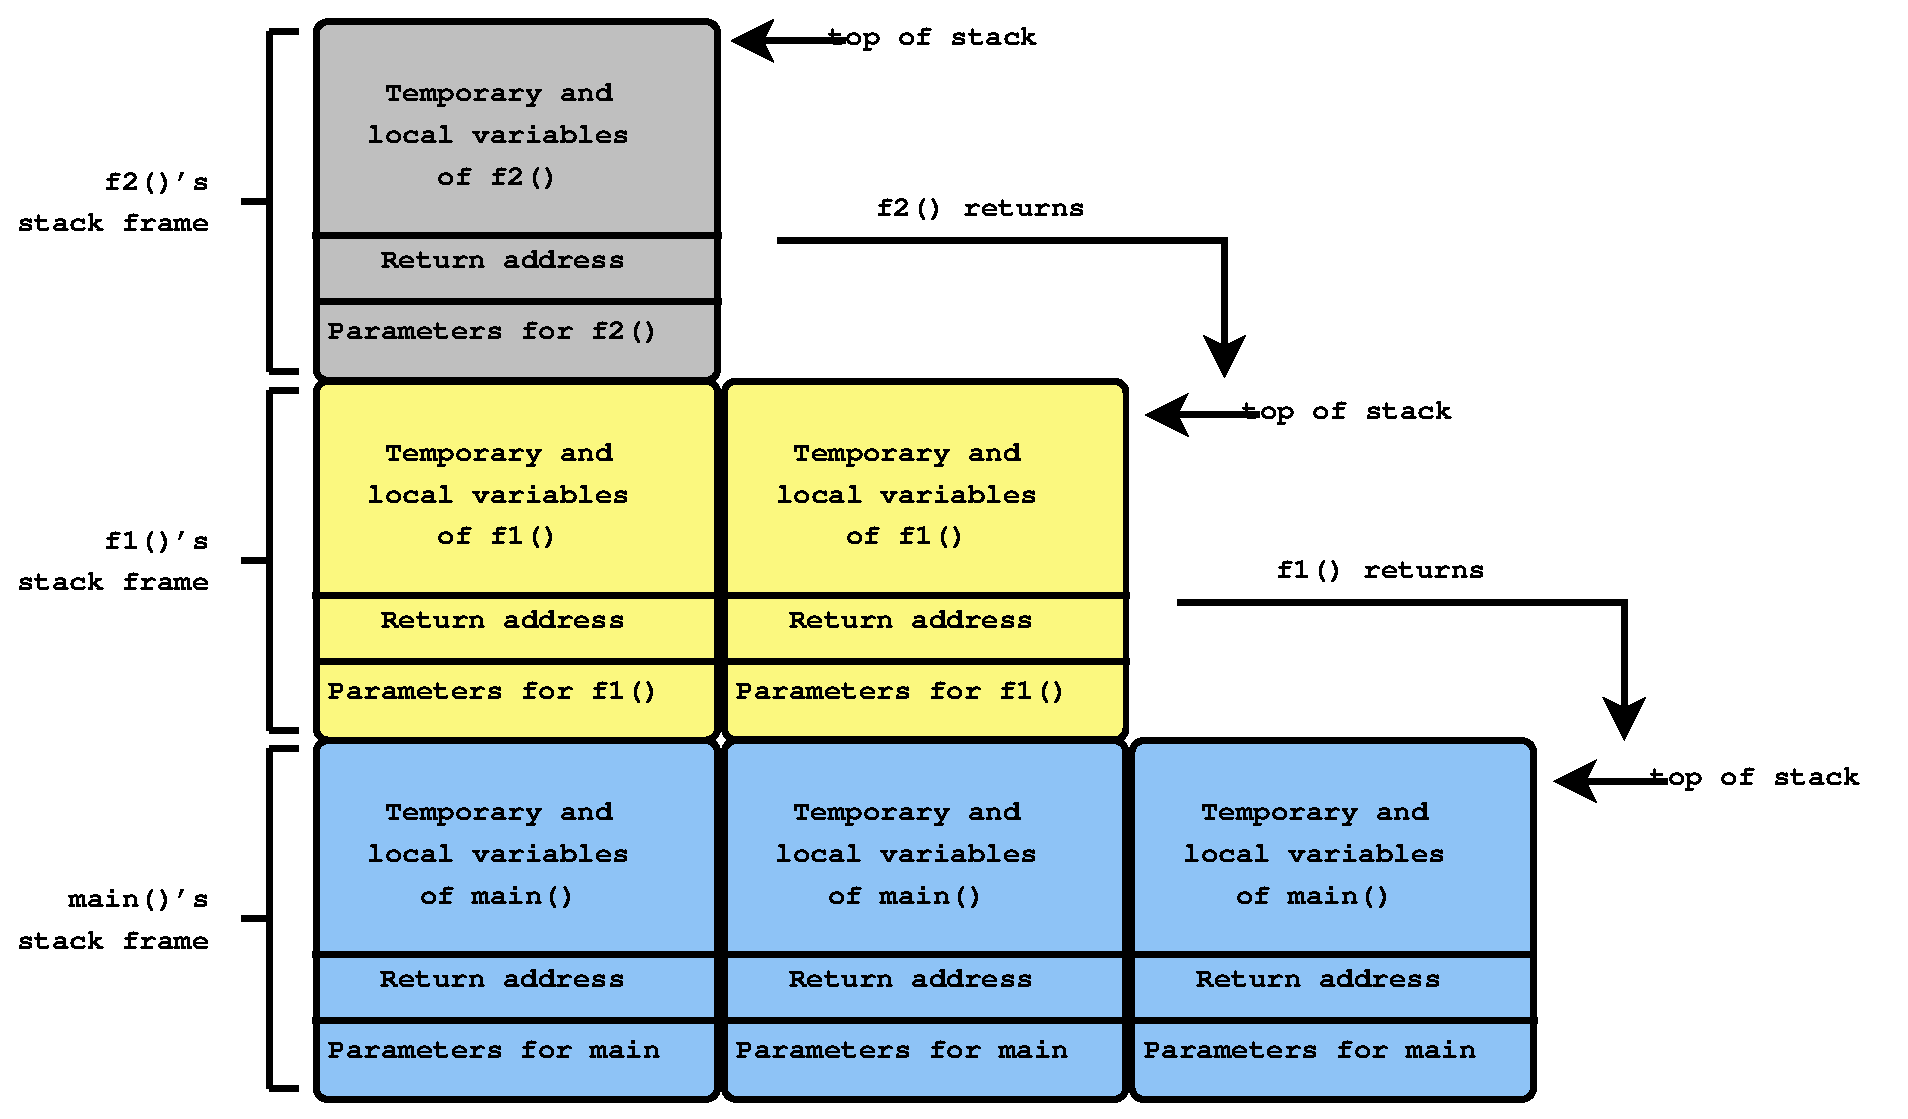
\includegraphics[width=0.8\textwidth]{src/img/stacklayout}
\caption{Typical stack layout}
\label{fig:stacklayout}
\end{figure}

Suppose we have a process whose current call chain is main()-f1()-f2(). The process's stack and its evolution follow something similar to Figure \ref{fig:stacklayout}.

The information contained in the stack at any point in time allows us to trace the call chain from the current execution point all the way to a program's entry point. Suppose that f2() in \ref{fig:stacklayout} did an allocation in which we were interested. By using the stack, we are able to go back from an allocation site through as many callers as we want. This answers one of our original questions: who is responsible for allocating memory?

